\section{Métodos para Problemas de Valor Inicial}

Um Problema de Valor Inicial, ou PVI, é caracterizado por uma equação diferencial acompanhada de uma condição imposta no início do intervalo de integração. Na forma escalar, considera-se

\[
    \frac{dy}{dt}=f(t,y), \qquad y(t_0)=y_0.
\]

Nos problemas implementados, a solução contínua foi substituída por uma sequência de aproximações calculadas em pontos igualmente espaçados. Essa escolha permite comparar métodos de diferentes ordens, observar a influência do passo \(h\) e validar numericamente os resultados por meio de soluções analíticas, quando disponíveis.

\subsection{Método de Euler Explícito}

\subsubsection{Fundamentação Teórica}

O Método de Euler Explícito é o procedimento mais direto entre os métodos estudados para PVI. A ideia central é aproximar a solução no próximo ponto usando apenas a inclinação da curva no ponto atual:

\[
    y_{n+1}=y_n+h f(t_n,y_n).
\]

Por utilizar uma única avaliação de \(f\) por passo, o método possui baixo custo computacional. Em contrapartida, seu erro tende a ser maior do que o dos métodos de ordem superior, pois a inclinação é considerada constante durante todo o subintervalo.

\subsubsection{Estratégia de Implementação}

A implementação foi feita manualmente em Python puro, usando listas para armazenar os tempos e os valores aproximados. A função recebe a equação diferencial, o tempo inicial, a condição inicial, o passo e o número de iterações. Em cada iteração, calcula-se a derivada no ponto corrente e atualiza-se a solução pela fórmula de Euler. Para sistemas de EDOs, a mesma lógica foi aplicada componente a componente, atualizando simultaneamente todas as variáveis do vetor de estado.

\subsubsection{Estrutura dos Arquivos de Entrada e Saída}

Os dados de entrada são definidos nos módulos da pasta \texttt{exercicios/}. Cada problema contém a função diferencial, as condições iniciais, o intervalo, o passo e, quando disponível, a solução analítica. As saídas são gravadas em \texttt{resultados/}, no formato CSV com codificação UTF-8, e em \texttt{graficos/}, no formato PNG.

\subsubsection{Problemas Teste}

\paragraph{Problema Teste 1: Exercício 12.3 -- velocidade com resistência do ar}

O primeiro problema teste utilizado para avaliar o Método de Euler Explícito corresponde ao modelo de velocidade de um corpo sujeito à resistência do ar proporcional à velocidade. A equação diferencial considerada é

\[
    \frac{dv}{dt}=\frac{2000-2v}{200-t},
\]

com condição inicial \(v(0)=0\), intervalo \(0\leq t\leq 50\) e solução analítica \(v(t)=10t-\frac{t^2}{40}\). Esse problema é adequado para validação porque permite comparar a solução numérica com um valor exato no ponto final, \(v(50)=437{,}5\).

Na implementação, o Método de Euler Explícito foi aplicado com passo \(h=1\), armazenando-se a evolução de \(v(t)\) ao longo do intervalo. Nesse caso, a aproximação usa apenas a inclinação no início de cada subintervalo, o que torna o procedimento simples, mas mais sensível ao tamanho do passo.

\begin{table}[H]
    \centering
    \caption{Resultados do Método de Euler Explícito no Exercício 12.3.}
    \begin{tabular}{c|r|r|r}
        \textbf{Passo} & \textbf{\(v_h(50)\)} & \textbf{\(v(50)\)} & \textbf{Erro absoluto} \\
        \hline
        \(h=5\) & 442{,}307692 & 437{,}500000 & 4{,}807692 \\
        \(h=2{,}5\) & 439{,}873418 & 437{,}500000 & 2{,}373418 \\
        \(h=1\) & 438{,}442211 & 437{,}500000 & 0{,}942211 \\
    \end{tabular}
\end{table}
% TODO: inserir figura específica do Método de Euler Explícito no Exercício 12.3

O valor final obtido pelo Método de Euler Explícito foi \(v(50)=438{,}442211\), com erro absoluto igual a \(0{,}942211\). A curva numérica acompanha a tendência crescente da solução exata; a diferença observada no ponto final expressa o erro acumulado durante o processo iterativo.

\paragraph{Problema Teste 2: Exercício 12.10 -- crescimento populacional}

O segundo problema teste corresponde ao modelo de crescimento populacional exponencial,

\[
    \frac{dp}{dt}=Gp,
\]

com \(p(0)=10000\), taxa \(G=0{,}075\), intervalo \(0\leq t\leq 20\) e passo \(h=0{,}5\). A solução analítica é \(p(t)=p_0e^{Gt}\), o que permite avaliar objetivamente a propagação do erro numérico ao longo do tempo.

O Método de Euler Explícito foi aplicado para estimar a população em cada ponto da malha temporal. Como a solução cresce exponencialmente, esse problema evidencia com clareza o efeito do erro acumulado: pequenas diferenças em passos intermediários podem se tornar mais visíveis no final do intervalo.

\begin{table}[H]
    \centering
    \caption{Resultados do Método de Euler Explícito no Exercício 12.10.}
    \begin{tabular}{c|r|r|r}
        \textbf{\(t\)} & \textbf{Aproximação} & \textbf{Solução exata} & \textbf{Erro absoluto} \\
        \hline
        0 & 10000{,}000000 & 10000{,}000000 & 0{,}000000 \\
        20 & 43603{,}787590 & 44816{,}890703 & 1213{,}103114 \\
    \end{tabular}
\end{table}
% TODO: inserir figura específica do Método de Euler Explícito no Exercício 12.10

No instante \(t=20\), o Método de Euler Explícito obteve \(p(20)=43603{,}787590\), enquanto a solução exata é \(44816{,}890703\). O erro absoluto final foi \(1213{,}103114\). Esse resultado permite discutir a precisão do método diante de uma solução monotonicamente crescente.

\paragraph{Problema Teste 3: Exercício 12.16 -- sistema hospedeiro-parasita}

O terceiro problema teste é um sistema acoplado do tipo Lotka-Volterra, usado para representar uma relação hospedeiro-parasita:

\[
    \frac{dH}{dt}=g_1H-d_1PH,
\]

\[
    \frac{dP}{dt}=-d_2P+g_2PH.
\]

Foram usados \(H(0)=20\), \(P(0)=5\), \(g_1=1\), \(d_1=0{,}1\), \(g_2=0{,}02\), \(d_2=0{,}5\), intervalo \(0\leq t\leq 2\) e passo \(h=0{,}01\). Nesse caso, o Método de Euler Explícito foi aplicado componente a componente, atualizando simultaneamente as populações \(H(t)\) e \(P(t)\).

\begin{table}[H]
    \centering
    \caption{Valores inicial e final do Método de Euler Explícito no Exercício 12.16.}
    \begin{tabular}{c|r|r}
        \textbf{\(t\)} & \textbf{\(H(t)\)} & \textbf{\(P(t)\)} \\
        \hline
        0{,}0 & 20{,}000000 & 5{,}000000 \\
        2{,}0 & 50{,}057446 & 7{,}101710 \\
    \end{tabular}
\end{table}
% TODO: inserir figura específica do Método de Euler Explícito no Exercício 12.16

Ao final da simulação, o Método de Euler Explícito produziu \(H(2)=50{,}057446\) e \(P(2)=7{,}101710\). A interpretação qualitativa é coerente com o modelo: os hospedeiros crescem durante o intervalo analisado, enquanto os parasitas apresentam resposta dependente da disponibilidade de hospedeiros.

\paragraph{Problema Teste 4: Modelo SEIAHR -- simulação epidêmica hipotética}

O quarto problema teste corresponde ao modelo epidêmico SEIAHR, composto pelos compartimentos \(S\), \(E\), \(I\), \(A\), \(H\), \(R\) e pela variável acumulada de mortes \(D\). O sistema foi simulado em \(0\leq t\leq 50\), com passo \(h=1\), considerando a forma normalizada da força de infecção, \(\lambda=\beta(I+A)/N\).

Os parâmetros usados foram \(\chi=0{,}6\), \(\alpha=0{,}33\), \(p=0{,}75\), \(\delta=0{,}1\), \(\phi=0{,}01\), \(\mu=0{,}03\), \(\beta=0{,}5\) e \(\rho=0{,}1\). A condição inicial foi \(S(0)=400000\), \(E(0)=0\), \(I(0)=1\), \(A(0)=0\), \(H(0)=0\), \(R(0)=0\) e \(D(0)=0\).

\begin{table}[H]
    \centering
    \caption{Estado final do Método de Euler Explícito no modelo SEIAHR normalizado.}
    \begin{tabular}{c|r|r|r|r}
        \textbf{Dia} & \textbf{\(S\)} & \textbf{\(I\)} & \textbf{\(H\)} & \textbf{\(D\)} \\
        \hline
        50 & 399943{,}791989 & 4{,}399613 & 0{,}022479 & 0{,}011220 \\
    \end{tabular}
\end{table}
% TODO: inserir figura específica do Método de Euler Explícito no modelo SEIAHR

No dia 50, o Método de Euler Explícito estimou \(I(50)=4{,}399613\), \(H(50)=0{,}022479\) e \(D(50)=0{,}011220\). A análise do resultado deve observar a coerência epidemiológica das trajetórias: suscetíveis não devem aumentar, recuperados e mortes acumuladas não devem decrescer, e \(D(t)\) deve ser interpretado separadamente de \(H(t)\).

\subsubsection{Validação dos Resultados}

A validação da implementação foi conduzida por meio da comparação entre a solução numérica e a solução analítica disponível. No Exercício 12.3, para \(h=1\), Euler obteve \(v(50)=438{,}442211\), enquanto o valor exato é \(437{,}5\), produzindo erro absoluto de \(0{,}942211\). No Exercício 12.10, Euler estimou \(p(20)=43603{,}787590\), contra \(44816{,}890703\) da solução exata. O erro absoluto, nesse caso, foi \(1213{,}103114\).

Observa-se que a redução do passo de integração resulta em diminuição consistente do erro no Exercício 12.3: para \(h=5\), o erro final foi \(4{,}807692\); para \(h=2{,}5\), passou a \(2{,}373418\); e, para \(h=1\), caiu para \(0{,}942211\). Esse comportamento indica convergência, embora o método permaneça menos preciso que os demais.

\subsubsection{Dificuldades Enfrentadas}

A principal dificuldade associada ao Método de Euler está no acúmulo de erro ao longo das iterações. Como a inclinação é calculada apenas no início do intervalo, o método pode subestimar ou superestimar a solução quando a função apresenta crescimento acentuado. Isso ficou evidente no crescimento populacional, em que a solução aproximada se afastou progressivamente da solução exponencial exata.

\subsection{Método de Euler Melhorado / Heun}

\subsubsection{Fundamentação Teórica}

O Método de Heun, também conhecido como Euler Melhorado, corrige uma limitação do Euler Explícito ao usar uma etapa preditora e uma etapa corretora. Primeiro calcula-se uma estimativa preliminar:

\[
    \widetilde{y}_{n+1}=y_n+h f(t_n,y_n).
\]

Em seguida, usa-se a média entre a inclinação inicial e a inclinação estimada no final do intervalo:

\[
    y_{n+1}=y_n+\frac{h}{2}\left[f(t_n,y_n)+f(t_{n+1},\widetilde{y}_{n+1})\right].
\]

Essa estrutura torna o método mais preciso que Euler, pois incorpora uma informação adicional sobre a variação da função no subintervalo.

\subsubsection{Estratégia de Implementação}

A implementação seguiu diretamente as duas etapas do método. Em cada passo, calcula-se a inclinação inicial, constrói-se o valor predito e, por fim, calcula-se a correção pela média das inclinações. Para sistemas, o mesmo procedimento foi aplicado a cada componente do vetor de estado, preservando o acoplamento entre as variáveis.

\subsubsection{Estrutura dos Arquivos de Entrada e Saída}

O método utiliza a mesma estrutura de entrada dos demais PVIs: função diferencial, intervalo, condição inicial e passo. Os resultados são exportados nas mesmas tabelas comparativas dos exercícios, o que permite avaliar Heun lado a lado com Euler, Ponto Médio e RK4.

\subsubsection{Problemas Teste}

\paragraph{Problema Teste 1: Exercício 12.3 -- velocidade com resistência do ar}

O primeiro problema teste utilizado para avaliar o Método de Heun corresponde ao modelo de velocidade de um corpo sujeito à resistência do ar proporcional à velocidade. A equação diferencial considerada é

\[
    \frac{dv}{dt}=\frac{2000-2v}{200-t},
\]

com condição inicial \(v(0)=0\), intervalo \(0\leq t\leq 50\) e solução analítica \(v(t)=10t-\frac{t^2}{40}\). Esse problema é adequado para validação porque permite comparar a solução numérica com um valor exato no ponto final, \(v(50)=437{,}5\).

Na implementação, o Método de Heun foi aplicado com passo \(h=1\), armazenando-se a evolução de \(v(t)\) ao longo do intervalo. Nesse caso, o cálculo envolve uma etapa preditora e uma etapa corretora, permitindo que a inclinação usada no avanço represente melhor o comportamento médio da solução no subintervalo.

\begin{table}[H]
    \centering
    \caption{Resultados do Método de Heun no Exercício 12.3.}
    \begin{tabular}{c|r|r|r}
        \textbf{Passo} & \textbf{\(v_h(50)\)} & \textbf{\(v(50)\)} & \textbf{Erro absoluto} \\
        \hline
        \(h=5\) & 437{,}357124 & 437{,}500000 & 0{,}142876 \\
        \(h=2{,}5\) & 437{,}465059 & 437{,}500000 & 0{,}034941 \\
        \(h=1\) & 437{,}494483 & 437{,}500000 & 0{,}005517 \\
    \end{tabular}
\end{table}
% TODO: inserir figura específica do Método de Heun no Exercício 12.3

O valor final obtido pelo Método de Heun foi \(v(50)=437{,}494483\), com erro absoluto igual a \(0{,}005517\). A curva numérica acompanha a tendência crescente da solução exata; a diferença observada no ponto final expressa o erro acumulado durante o processo iterativo.

\paragraph{Problema Teste 2: Exercício 12.10 -- crescimento populacional}

O segundo problema teste corresponde ao modelo de crescimento populacional exponencial,

\[
    \frac{dp}{dt}=Gp,
\]

com \(p(0)=10000\), taxa \(G=0{,}075\), intervalo \(0\leq t\leq 20\) e passo \(h=0{,}5\). A solução analítica é \(p(t)=p_0e^{Gt}\), o que permite avaliar objetivamente a propagação do erro numérico ao longo do tempo.

O Método de Heun foi aplicado para estimar a população em cada ponto da malha temporal. Como a solução cresce exponencialmente, esse problema evidencia com clareza o efeito do erro acumulado: pequenas diferenças em passos intermediários podem se tornar mais visíveis no final do intervalo.

\begin{table}[H]
    \centering
    \caption{Resultados do Método de Heun no Exercício 12.10.}
    \begin{tabular}{c|r|r|r}
        \textbf{\(t\)} & \textbf{Aproximação} & \textbf{Solução exata} & \textbf{Erro absoluto} \\
        \hline
        0 & 10000{,}000000 & 10000{,}000000 & 0{,}000000 \\
        20 & 44801{,}573875 & 44816{,}890703 & 15{,}316828 \\
    \end{tabular}
\end{table}
% TODO: inserir figura específica do Método de Heun no Exercício 12.10

No instante \(t=20\), o Método de Heun obteve \(p(20)=44801{,}573875\), enquanto a solução exata é \(44816{,}890703\). O erro absoluto final foi \(15{,}316828\). Esse resultado permite discutir a precisão do método diante de uma solução monotonicamente crescente.

\paragraph{Problema Teste 3: Exercício 12.16 -- sistema hospedeiro-parasita}

O terceiro problema teste é um sistema acoplado do tipo Lotka-Volterra, usado para representar uma relação hospedeiro-parasita:

\[
    \frac{dH}{dt}=g_1H-d_1PH,
\]

\[
    \frac{dP}{dt}=-d_2P+g_2PH.
\]

Foram usados \(H(0)=20\), \(P(0)=5\), \(g_1=1\), \(d_1=0{,}1\), \(g_2=0{,}02\), \(d_2=0{,}5\), intervalo \(0\leq t\leq 2\) e passo \(h=0{,}01\). Nesse caso, o Método de Heun foi aplicado componente a componente, atualizando simultaneamente as populações \(H(t)\) e \(P(t)\).

\begin{table}[H]
    \centering
    \caption{Valores inicial e final do Método de Heun no Exercício 12.16.}
    \begin{tabular}{c|r|r}
        \textbf{\(t\)} & \textbf{\(H(t)\)} & \textbf{\(P(t)\)} \\
        \hline
        0{,}0 & 20{,}000000 & 5{,}000000 \\
        2{,}0 & 50{,}006439 & 7{,}131074 \\
    \end{tabular}
\end{table}
% TODO: inserir figura específica do Método de Heun no Exercício 12.16

Ao final da simulação, o Método de Heun produziu \(H(2)=50{,}006439\) e \(P(2)=7{,}131074\). A interpretação qualitativa é coerente com o modelo: os hospedeiros crescem durante o intervalo analisado, enquanto os parasitas apresentam resposta dependente da disponibilidade de hospedeiros.

\paragraph{Problema Teste 4: Modelo SEIAHR -- simulação epidêmica hipotética}

O quarto problema teste corresponde ao modelo epidêmico SEIAHR, composto pelos compartimentos \(S\), \(E\), \(I\), \(A\), \(H\), \(R\) e pela variável acumulada de mortes \(D\). O sistema foi simulado em \(0\leq t\leq 50\), com passo \(h=1\), considerando a forma normalizada da força de infecção, \(\lambda=\beta(I+A)/N\).

Os parâmetros usados foram \(\chi=0{,}6\), \(\alpha=0{,}33\), \(p=0{,}75\), \(\delta=0{,}1\), \(\phi=0{,}01\), \(\mu=0{,}03\), \(\beta=0{,}5\) e \(\rho=0{,}1\). A condição inicial foi \(S(0)=400000\), \(E(0)=0\), \(I(0)=1\), \(A(0)=0\), \(H(0)=0\), \(R(0)=0\) e \(D(0)=0\).

\begin{table}[H]
    \centering
    \caption{Estado final do Método de Heun no modelo SEIAHR normalizado.}
    \begin{tabular}{c|r|r|r|r}
        \textbf{Dia} & \textbf{\(S\)} & \textbf{\(I\)} & \textbf{\(H\)} & \textbf{\(D\)} \\
        \hline
        50 & 399943{,}213736 & 4{,}879833 & 0{,}024944 & 0{,}012312 \\
    \end{tabular}
\end{table}
% TODO: inserir figura específica do Método de Heun no modelo SEIAHR

No dia 50, o Método de Heun estimou \(I(50)=4{,}879833\), \(H(50)=0{,}024944\) e \(D(50)=0{,}012312\). A análise do resultado deve observar a coerência epidemiológica das trajetórias: suscetíveis não devem aumentar, recuperados e mortes acumuladas não devem decrescer, e \(D(t)\) deve ser interpretado separadamente de \(H(t)\).

\subsubsection{Validação dos Resultados}

No Exercício 12.3, para \(h=1\), Heun obteve \(v(50)=437{,}494483\), com erro absoluto de \(0{,}005517\). No Exercício 12.10, produziu \(p(20)=44801{,}573875\), com erro absoluto de \(15{,}316828\). Esses valores são substancialmente melhores que os de Euler, confirmando o ganho esperado para um método de segunda ordem.

A consistência dos resultados também foi verificada pela proximidade entre Heun e Ponto Médio. No modelo SEIAHR, Heun estimou \(I(50)=4{,}879833\), valor muito próximo ao resultado do Ponto Médio e do RK4, indicando comportamento numérico coerente.

\subsubsection{Dificuldades Enfrentadas}

A principal atenção na implementação de Heun foi garantir que o valor predito fosse usado apenas para calcular a segunda inclinação, sem substituir prematuramente o estado atual. Em sistemas acoplados, essa distinção é importante porque todas as componentes devem ser corrigidas a partir do mesmo vetor predito.

\subsection{Método do Ponto Médio}

\subsubsection{Fundamentação Teórica}

O Método do Ponto Médio estima a inclinação no centro do subintervalo. Sua formulação é dada por

\[
    k_1=f(t_n,y_n),
\]

\[
    k_2=f\left(t_n+\frac{h}{2},y_n+\frac{h}{2}k_1\right),
\]

\[
    y_{n+1}=y_n+h k_2.
\]

Como Heun, trata-se de um método de segunda ordem. A diferença está na escolha da inclinação representativa: em vez de usar a média entre início e fim, usa-se uma inclinação calculada no ponto médio estimado.

\subsubsection{Estratégia de Implementação}

O algoritmo calcula inicialmente \(k_1\), usa essa inclinação para estimar o estado intermediário e, então, avalia \(k_2\). O avanço do passo é feito com base em \(k_2\). Nos sistemas, a estimativa intermediária é calculada para todas as componentes antes da avaliação final da derivada.

\subsubsection{Estrutura dos Arquivos de Entrada e Saída}

As entradas são compartilhadas com os demais métodos de PVI. As saídas são organizadas nas tabelas comparativas de cada exercício, incluindo aproximações, erro absoluto e erro relativo quando há solução analítica.

\subsubsection{Problemas Teste}

\paragraph{Problema Teste 1: Exercício 12.3 -- velocidade com resistência do ar}

O primeiro problema teste utilizado para avaliar o Método do Ponto Médio corresponde ao modelo de velocidade de um corpo sujeito à resistência do ar proporcional à velocidade. A equação diferencial considerada é

\[
    \frac{dv}{dt}=\frac{2000-2v}{200-t},
\]

com condição inicial \(v(0)=0\), intervalo \(0\leq t\leq 50\) e solução analítica \(v(t)=10t-\frac{t^2}{40}\). Esse problema é adequado para validação porque permite comparar a solução numérica com um valor exato no ponto final, \(v(50)=437{,}5\).

Na implementação, o Método do Ponto Médio foi aplicado com passo \(h=1\), armazenando-se a evolução de \(v(t)\) ao longo do intervalo. Nesse caso, calcula-se uma inclinação intermediária no centro do subintervalo, e essa inclinação passa a representar o avanço da solução no passo considerado.

\begin{table}[H]
    \centering
    \caption{Resultados do Método do Ponto Médio no Exercício 12.3.}
    \begin{tabular}{c|r|r|r}
        \textbf{Passo} & \textbf{\(v_h(50)\)} & \textbf{\(v(50)\)} & \textbf{Erro absoluto} \\
        \hline
        \(h=5\) & 437{,}429615 & 437{,}500000 & 0{,}070385 \\
        \(h=2{,}5\) & 437{,}482658 & 437{,}500000 & 0{,}017342 \\
        \(h=1\) & 437{,}497250 & 437{,}500000 & 0{,}002750 \\
    \end{tabular}
\end{table}
% TODO: inserir figura específica do Método do Ponto Médio no Exercício 12.3

O valor final obtido pelo Método do Ponto Médio foi \(v(50)=437{,}497250\), com erro absoluto igual a \(0{,}002750\). A curva numérica acompanha a tendência crescente da solução exata; a diferença observada no ponto final expressa o erro acumulado durante o processo iterativo.

\paragraph{Problema Teste 2: Exercício 12.10 -- crescimento populacional}

O segundo problema teste corresponde ao modelo de crescimento populacional exponencial,

\[
    \frac{dp}{dt}=Gp,
\]

com \(p(0)=10000\), taxa \(G=0{,}075\), intervalo \(0\leq t\leq 20\) e passo \(h=0{,}5\). A solução analítica é \(p(t)=p_0e^{Gt}\), o que permite avaliar objetivamente a propagação do erro numérico ao longo do tempo.

O Método do Ponto Médio foi aplicado para estimar a população em cada ponto da malha temporal. Como a solução cresce exponencialmente, esse problema evidencia com clareza o efeito do erro acumulado: pequenas diferenças em passos intermediários podem se tornar mais visíveis no final do intervalo.

\begin{table}[H]
    \centering
    \caption{Resultados do Método do Ponto Médio no Exercício 12.10.}
    \begin{tabular}{c|r|r|r}
        \textbf{\(t\)} & \textbf{Aproximação} & \textbf{Solução exata} & \textbf{Erro absoluto} \\
        \hline
        0 & 10000{,}000000 & 10000{,}000000 & 0{,}000000 \\
        20 & 44801{,}573875 & 44816{,}890703 & 15{,}316828 \\
    \end{tabular}
\end{table}
% TODO: inserir figura específica do Método do Ponto Médio no Exercício 12.10

No instante \(t=20\), o Método do Ponto Médio obteve \(p(20)=44801{,}573875\), enquanto a solução exata é \(44816{,}890703\). O erro absoluto final foi \(15{,}316828\). Esse resultado permite discutir a precisão do método diante de uma solução monotonicamente crescente.

\paragraph{Problema Teste 3: Exercício 12.16 -- sistema hospedeiro-parasita}

O terceiro problema teste é um sistema acoplado do tipo Lotka-Volterra, usado para representar uma relação hospedeiro-parasita:

\[
    \frac{dH}{dt}=g_1H-d_1PH,
\]

\[
    \frac{dP}{dt}=-d_2P+g_2PH.
\]

Foram usados \(H(0)=20\), \(P(0)=5\), \(g_1=1\), \(d_1=0{,}1\), \(g_2=0{,}02\), \(d_2=0{,}5\), intervalo \(0\leq t\leq 2\) e passo \(h=0{,}01\). Nesse caso, o Método do Ponto Médio foi aplicado componente a componente, atualizando simultaneamente as populações \(H(t)\) e \(P(t)\).

\begin{table}[H]
    \centering
    \caption{Valores inicial e final do Método do Ponto Médio no Exercício 12.16.}
    \begin{tabular}{c|r|r}
        \textbf{\(t\)} & \textbf{\(H(t)\)} & \textbf{\(P(t)\)} \\
        \hline
        0{,}0 & 20{,}000000 & 5{,}000000 \\
        2{,}0 & 50{,}006576 & 7{,}131060 \\
    \end{tabular}
\end{table}
% TODO: inserir figura específica do Método do Ponto Médio no Exercício 12.16

Ao final da simulação, o Método do Ponto Médio produziu \(H(2)=50{,}006576\) e \(P(2)=7{,}131060\). A interpretação qualitativa é coerente com o modelo: os hospedeiros crescem durante o intervalo analisado, enquanto os parasitas apresentam resposta dependente da disponibilidade de hospedeiros.

\paragraph{Problema Teste 4: Modelo SEIAHR -- simulação epidêmica hipotética}

O quarto problema teste corresponde ao modelo epidêmico SEIAHR, composto pelos compartimentos \(S\), \(E\), \(I\), \(A\), \(H\), \(R\) e pela variável acumulada de mortes \(D\). O sistema foi simulado em \(0\leq t\leq 50\), com passo \(h=1\), considerando a forma normalizada da força de infecção, \(\lambda=\beta(I+A)/N\).

Os parâmetros usados foram \(\chi=0{,}6\), \(\alpha=0{,}33\), \(p=0{,}75\), \(\delta=0{,}1\), \(\phi=0{,}01\), \(\mu=0{,}03\), \(\beta=0{,}5\) e \(\rho=0{,}1\). A condição inicial foi \(S(0)=400000\), \(E(0)=0\), \(I(0)=1\), \(A(0)=0\), \(H(0)=0\), \(R(0)=0\) e \(D(0)=0\).

\begin{table}[H]
    \centering
    \caption{Estado final do Método do Ponto Médio no modelo SEIAHR normalizado.}
    \begin{tabular}{c|r|r|r|r}
        \textbf{Dia} & \textbf{\(S\)} & \textbf{\(I\)} & \textbf{\(H\)} & \textbf{\(D\)} \\
        \hline
        50 & 399943{,}213730 & 4{,}879834 & 0{,}024944 & 0{,}012312 \\
    \end{tabular}
\end{table}
% TODO: inserir figura específica do Método do Ponto Médio no modelo SEIAHR

No dia 50, o Método do Ponto Médio estimou \(I(50)=4{,}879834\), \(H(50)=0{,}024944\) e \(D(50)=0{,}012312\). A análise do resultado deve observar a coerência epidemiológica das trajetórias: suscetíveis não devem aumentar, recuperados e mortes acumuladas não devem decrescer, e \(D(t)\) deve ser interpretado separadamente de \(H(t)\).

\subsubsection{Validação dos Resultados}

No Exercício 12.3, com \(h=1\), o Ponto Médio obteve \(v(50)=437{,}497250\), com erro absoluto de \(0{,}002750\). No Exercício 12.10, produziu o mesmo valor registrado para Heun no instante final, \(p(20)=44801{,}573875\), com erro absoluto de \(15{,}316828\). A proximidade com Heun é compatível com a teoria, pois ambos usam duas avaliações da função por passo.

No Exercício 12.16, o Ponto Médio chegou a \(H(2)=50{,}006576\) e \(P(2)=7{,}131060\), muito próximo do RK4. Essa proximidade indica estabilidade para o passo \(h=0{,}01\).

\subsubsection{Dificuldades Enfrentadas}

A principal dificuldade foi preservar a interpretação correta do ponto médio em sistemas. O estado intermediário não é solução final do passo; ele serve apenas para estimar a inclinação que representa melhor o subintervalo.

\subsection{Método de Runge-Kutta de Quarta Ordem}

\subsubsection{Fundamentação Teórica}

O método de Runge-Kutta de quarta ordem, ou RK4, utiliza quatro avaliações da função diferencial para construir uma média ponderada das inclinações:

\[
    y_{n+1}=y_n+\frac{h}{6}(k_1+2k_2+2k_3+k_4).
\]

As inclinações \(k_1\), \(k_2\), \(k_3\) e \(k_4\) são avaliadas no início, em dois pontos intermediários e no final do subintervalo. Essa composição reduz significativamente o erro local, tornando o método adequado como referência numérica nos problemas deste relatório.

\subsubsection{Estratégia de Implementação}

A implementação calcula sequencialmente as quatro inclinações e atualiza a solução pela média ponderada. Em sistemas, cada \(k\) é um vetor, e a combinação ponderada é feita componente a componente, sem uso de bibliotecas vetoriais.

\subsubsection{Estrutura dos Arquivos de Entrada e Saída}

O RK4 usa os mesmos arquivos de entrada dos demais métodos e aparece nas tabelas comparativas como método de maior ordem. Nos gráficos finais dos sistemas, ele foi usado como referência principal por apresentar maior estabilidade e precisão.

\subsubsection{Problemas Teste}

\paragraph{Problema Teste 1: Exercício 12.3 -- velocidade com resistência do ar}

O primeiro problema teste utilizado para avaliar o Método de Runge-Kutta de Quarta Ordem corresponde ao modelo de velocidade de um corpo sujeito à resistência do ar proporcional à velocidade. A equação diferencial considerada é

\[
    \frac{dv}{dt}=\frac{2000-2v}{200-t},
\]

com condição inicial \(v(0)=0\), intervalo \(0\leq t\leq 50\) e solução analítica \(v(t)=10t-\frac{t^2}{40}\). Esse problema é adequado para validação porque permite comparar a solução numérica com um valor exato no ponto final, \(v(50)=437{,}5\).

Na implementação, o Método de Runge-Kutta de Quarta Ordem foi aplicado com passo \(h=1\), armazenando-se a evolução de \(v(t)\) ao longo do intervalo. Nesse caso, quatro inclinações são calculadas em posições distintas do subintervalo, e a média ponderada dessas inclinações fornece uma aproximação de maior ordem.

\begin{table}[H]
    \centering
    \caption{Resultados do Método de Runge-Kutta de Quarta Ordem no Exercício 12.3.}
    \begin{tabular}{c|r|r|r}
        \textbf{Passo} & \textbf{\(v_h(50)\)} & \textbf{\(v(50)\)} & \textbf{Erro absoluto} \\
        \hline
        \(h=5\) & 437{,}499969 & 437{,}500000 & 0{,}000031 \\
        \(h=2{,}5\) & 437{,}499998 & 437{,}500000 & 0{,}000002 \\
        \(h=1\) & 437{,}500000 & 437{,}500000 & 0{,}000000 \\
    \end{tabular}
\end{table}
% TODO: inserir figura específica do Método de Runge-Kutta de Quarta Ordem no Exercício 12.3

O valor final obtido pelo Método de Runge-Kutta de Quarta Ordem foi \(v(50)=437{,}500000\), com erro absoluto igual a \(0{,}000000\). A curva numérica acompanha a tendência crescente da solução exata; a diferença observada no ponto final expressa o erro acumulado durante o processo iterativo.

\paragraph{Problema Teste 2: Exercício 12.10 -- crescimento populacional}

O segundo problema teste corresponde ao modelo de crescimento populacional exponencial,

\[
    \frac{dp}{dt}=Gp,
\]

com \(p(0)=10000\), taxa \(G=0{,}075\), intervalo \(0\leq t\leq 20\) e passo \(h=0{,}5\). A solução analítica é \(p(t)=p_0e^{Gt}\), o que permite avaliar objetivamente a propagação do erro numérico ao longo do tempo.

O Método de Runge-Kutta de Quarta Ordem foi aplicado para estimar a população em cada ponto da malha temporal. Como a solução cresce exponencialmente, esse problema evidencia com clareza o efeito do erro acumulado: pequenas diferenças em passos intermediários podem se tornar mais visíveis no final do intervalo.

\begin{table}[H]
    \centering
    \caption{Resultados do Método de Runge-Kutta de Quarta Ordem no Exercício 12.10.}
    \begin{tabular}{c|r|r|r}
        \textbf{\(t\)} & \textbf{Aproximação} & \textbf{Solução exata} & \textbf{Erro absoluto} \\
        \hline
        0 & 10000{,}000000 & 10000{,}000000 & 0{,}000000 \\
        20 & 44816{,}889630 & 44816{,}890703 & 0{,}001074 \\
    \end{tabular}
\end{table}
% TODO: inserir figura específica do Método de Runge-Kutta de Quarta Ordem no Exercício 12.10

No instante \(t=20\), o Método de Runge-Kutta de Quarta Ordem obteve \(p(20)=44816{,}889630\), enquanto a solução exata é \(44816{,}890703\). O erro absoluto final foi \(0{,}001074\). Esse resultado permite discutir a precisão do método diante de uma solução monotonicamente crescente.

\paragraph{Problema Teste 3: Exercício 12.16 -- sistema hospedeiro-parasita}

O terceiro problema teste é um sistema acoplado do tipo Lotka-Volterra, usado para representar uma relação hospedeiro-parasita:

\[
    \frac{dH}{dt}=g_1H-d_1PH,
\]

\[
    \frac{dP}{dt}=-d_2P+g_2PH.
\]

Foram usados \(H(0)=20\), \(P(0)=5\), \(g_1=1\), \(d_1=0{,}1\), \(g_2=0{,}02\), \(d_2=0{,}5\), intervalo \(0\leq t\leq 2\) e passo \(h=0{,}01\). Nesse caso, o Método de Runge-Kutta de Quarta Ordem foi aplicado componente a componente, atualizando simultaneamente as populações \(H(t)\) e \(P(t)\).

\begin{table}[H]
    \centering
    \caption{Valores inicial e final do Método de Runge-Kutta de Quarta Ordem no Exercício 12.16.}
    \begin{tabular}{c|r|r}
        \textbf{\(t\)} & \textbf{\(H(t)\)} & \textbf{\(P(t)\)} \\
        \hline
        0{,}0 & 20{,}000000 & 5{,}000000 \\
        2{,}0 & 50{,}006193 & 7{,}131075 \\
    \end{tabular}
\end{table}
% TODO: inserir figura específica do Método de Runge-Kutta de Quarta Ordem no Exercício 12.16

Ao final da simulação, o Método de Runge-Kutta de Quarta Ordem produziu \(H(2)=50{,}006193\) e \(P(2)=7{,}131075\). A interpretação qualitativa é coerente com o modelo: os hospedeiros crescem durante o intervalo analisado, enquanto os parasitas apresentam resposta dependente da disponibilidade de hospedeiros.

\paragraph{Problema Teste 4: Modelo SEIAHR -- simulação epidêmica hipotética}

O quarto problema teste corresponde ao modelo epidêmico SEIAHR, composto pelos compartimentos \(S\), \(E\), \(I\), \(A\), \(H\), \(R\) e pela variável acumulada de mortes \(D\). O sistema foi simulado em \(0\leq t\leq 50\), com passo \(h=1\), considerando a forma normalizada da força de infecção, \(\lambda=\beta(I+A)/N\).

Os parâmetros usados foram \(\chi=0{,}6\), \(\alpha=0{,}33\), \(p=0{,}75\), \(\delta=0{,}1\), \(\phi=0{,}01\), \(\mu=0{,}03\), \(\beta=0{,}5\) e \(\rho=0{,}1\). A condição inicial foi \(S(0)=400000\), \(E(0)=0\), \(I(0)=1\), \(A(0)=0\), \(H(0)=0\), \(R(0)=0\) e \(D(0)=0\).

\begin{table}[H]
    \centering
    \caption{Estado final do Método de Runge-Kutta de Quarta Ordem no modelo SEIAHR normalizado.}
    \begin{tabular}{c|r|r|r|r}
        \textbf{Dia} & \textbf{\(S\)} & \textbf{\(I\)} & \textbf{\(H\)} & \textbf{\(D\)} \\
        \hline
        50 & 399943{,}190489 & 4{,}891144 & 0{,}025001 & 0{,}012338 \\
    \end{tabular}
\end{table}
% TODO: inserir figura específica do Método de Runge-Kutta de Quarta Ordem no modelo SEIAHR

No dia 50, o Método de Runge-Kutta de Quarta Ordem estimou \(I(50)=4{,}891144\), \(H(50)=0{,}025001\) e \(D(50)=0{,}012338\). A análise do resultado deve observar a coerência epidemiológica das trajetórias: suscetíveis não devem aumentar, recuperados e mortes acumuladas não devem decrescer, e \(D(t)\) deve ser interpretado separadamente de \(H(t)\).

\subsubsection{Validação dos Resultados}

No Exercício 12.3, o RK4 obteve \(v(50)=437{,}499969\) com \(h=5\), \(437{,}499998\) com \(h=2{,}5\) e \(437{,}500000\) com \(h=1\). A redução do erro ao diminuir o passo confirma a convergência do método. No Exercício 12.10, o erro absoluto final foi de apenas \(0{,}001074\), praticamente coincidindo com a solução analítica.

No sistema hospedeiro-parasita, os valores finais do RK4 ficaram próximos dos métodos de segunda ordem, o que indica estabilidade para o passo usado. No SEIAHR normalizado, o RK4 manteve comportamento coerente nos compartimentos epidemiológicos. A validação, nesse caso, foi feita por coerência qualitativa: os suscetíveis diminuem lentamente, recuperados e mortes acumuladas não decrescem, e os compartimentos permanecem em escala compatível com a simulação normalizada.

\subsubsection{Dificuldades Enfrentadas}

O maior cuidado no RK4 foi evitar misturar estados intermediários com o estado definitivo do passo. Como cada inclinação depende de uma estimativa específica, qualquer troca na ordem dos cálculos comprometeria a precisão do método.

\subsection{Análise Comparativa dos Métodos para Problemas de Valor Inicial}

\subsubsection{Avaliação no Exercício 12.3}

No Exercício 12.3, a solução exata \(v(t)=10t-\frac{t^2}{40}\) permitiu avaliar diretamente os erros. A Tabela \ref{tab:ex123-final} apresenta os valores finais em \(t=50\).

\begin{table}[H]
    \centering
    \caption{Valores finais no Exercício 12.3.}
    \label{tab:ex123-final}
    \begin{tabular}{c|r|r|r|r}
        \textbf{Passo} & \textbf{Euler} & \textbf{Heun} & \textbf{Ponto Médio} & \textbf{RK4} \\
        \hline
        \(h=5\) & 442{,}307692 & 437{,}357124 & 437{,}429615 & 437{,}499969 \\
        \(h=2{,}5\) & 439{,}873418 & 437{,}465059 & 437{,}482658 & 437{,}499998 \\
        \(h=1\) & 438{,}442211 & 437{,}494483 & 437{,}497250 & 437{,}500000 \\
    \end{tabular}
\end{table}

A redução de \(h\) diminuiu o erro de todos os métodos. Euler apresentou os maiores desvios, enquanto RK4 permaneceu praticamente sobre a solução exata.

\begin{table}[H]
    \centering
    \caption{Erros absolutos finais no Exercício 12.3.}
    \label{tab:ex123-erros}
    \begin{tabular}{c|r|r|r|r}
        \textbf{Passo} & \textbf{Euler} & \textbf{Heun} & \textbf{Ponto Médio} & \textbf{RK4} \\
        \hline
        \(h=5\) & 4{,}807692 & 0{,}142876 & 0{,}070385 & 0{,}000031 \\
        \(h=2{,}5\) & 2{,}373418 & 0{,}034941 & 0{,}017342 & 0{,}000002 \\
        \(h=1\) & 0{,}942211 & 0{,}005517 & 0{,}002750 & 0{,}000000 \\
    \end{tabular}
\end{table}

A Tabela \ref{tab:ex123-erros} deixa explícita a ordem qualitativa de precisão. A queda do erro ocorre em todos os métodos, mas é muito mais acentuada nos métodos de maior ordem. Esse resultado reforça que a validação não foi baseada apenas no valor final isolado, mas também no comportamento dos erros quando a malha é refinada.

\begin{figure}[H]
    \centering
    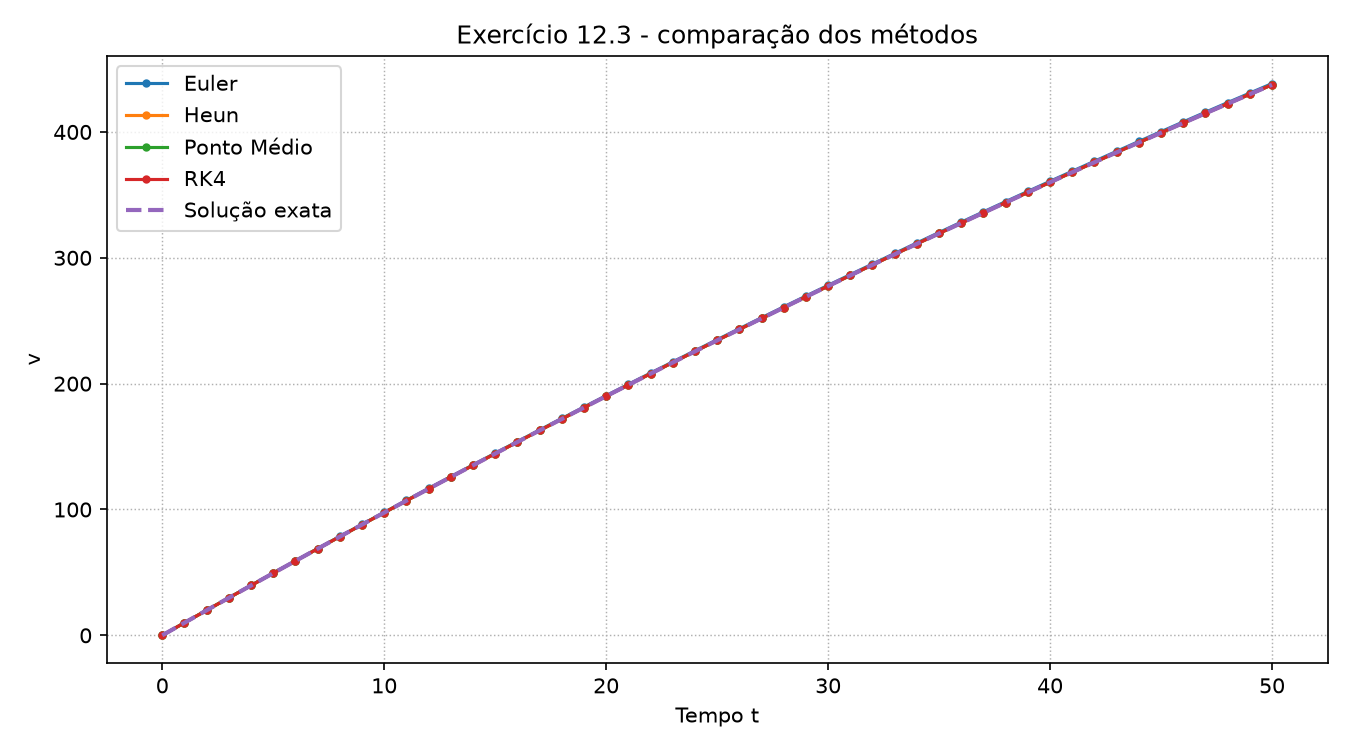
\includegraphics[width=0.85\textwidth]{../graficos/exercicio_12_3_h_1_0.png}
    \caption{Comparação dos métodos no Exercício 12.3 com \(h=1\).}
\end{figure}

% TODO: inserir gráfico de erro absoluto do Exercício 12.3 gerado pelo código

\subsubsection{Avaliação no Exercício 12.10}

No crescimento populacional, a solução exata no instante final foi \(44816{,}890703\). Euler estimou \(43603{,}787590\), Heun e Ponto Médio estimaram \(44801{,}573875\), e RK4 estimou \(44816{,}889630\). A comparação mostra que o erro de Euler cresce com o tempo em razão do caráter exponencial do problema. Os métodos de segunda ordem reduzem esse afastamento, e RK4 apresenta a melhor aproximação.

\begin{table}[H]
    \centering
    \caption{Valores e erros finais no Exercício 12.10.}
    \label{tab:ex1210-erros}
    \begin{tabular}{l|r|r}
        \textbf{Método} & \textbf{\(p_h(20)\)} & \textbf{Erro absoluto} \\
        \hline
        Euler & 43603{,}787590 & 1213{,}103114 \\
        Heun & 44801{,}573875 & 15{,}316828 \\
        Ponto Médio & 44801{,}573875 & 15{,}316828 \\
        RK4 & 44816{,}889630 & 0{,}001074 \\
    \end{tabular}
\end{table}

A diferença entre Euler e os demais métodos é particularmente visível nesse exercício porque a solução é acumulativa. Quando a inclinação é subestimada no início de cada subintervalo, o erro não fica restrito ao passo em que foi produzido; ele passa a compor a condição inicial do passo seguinte.

\begin{figure}[H]
    \centering
    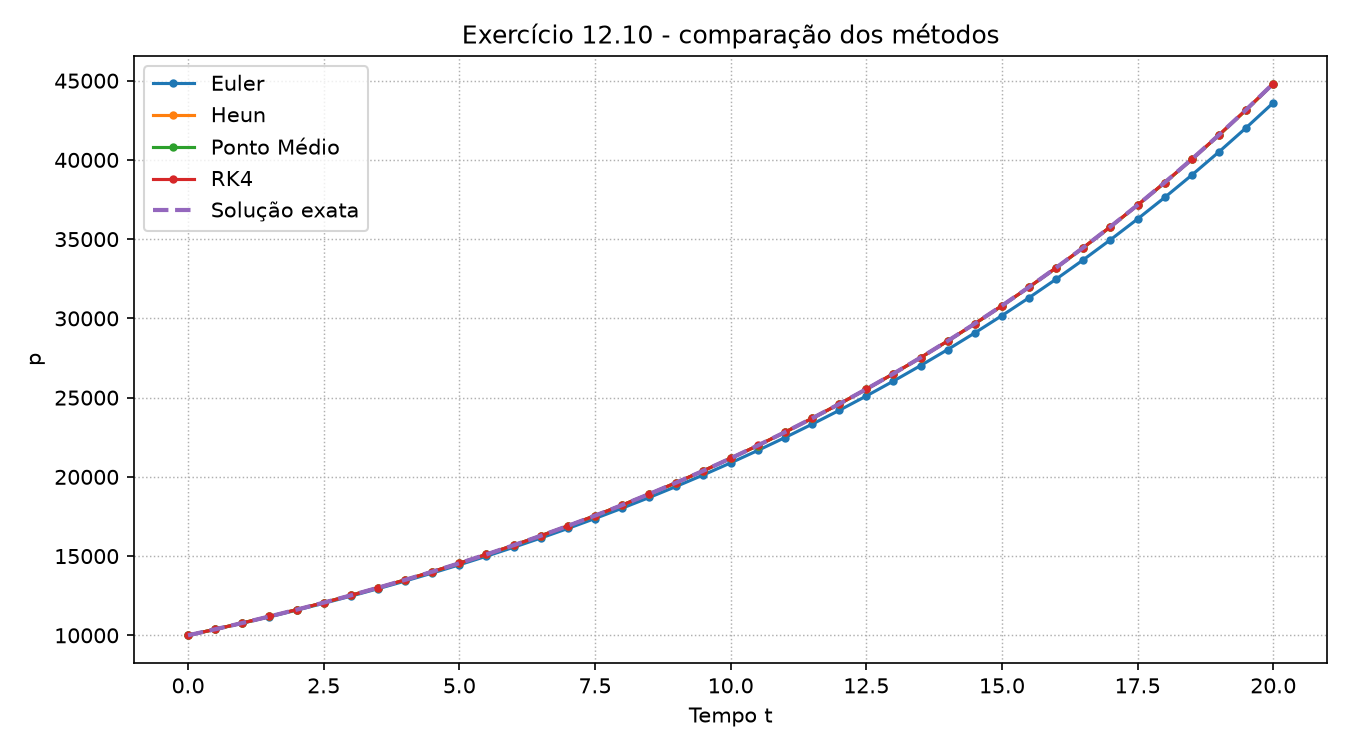
\includegraphics[width=0.85\textwidth]{../graficos/exercicio_12_10.png}
    \caption{Crescimento populacional do Exercício 12.10.}
\end{figure}

% TODO: inserir gráfico de erro absoluto do Exercício 12.10 gerado pelo código

\subsubsection{Avaliação no Exercício 12.16}

No sistema hospedeiro-parasita, a validação não dependeu de solução analítica, mas de comparação entre métodos e coerência qualitativa. Os valores selecionados pelo RK4 são apresentados na Tabela \ref{tab:ex1216-rk4}. A trajetória mostra crescimento dos hospedeiros e queda inicial seguida de crescimento dos parasitas, comportamento compatível com o acoplamento do modelo.

\begin{table}[H]
    \centering
    \caption{Valores selecionados do Exercício 12.16 pelo método RK4.}
    \label{tab:ex1216-rk4}
    \begin{tabular}{c|r|r}
        \textbf{\(t\)} & \textbf{Hospedeiros \(H\)} & \textbf{Parasitas \(P\)} \\
        \hline
        0{,}0 & 20{,}000000 & 5{,}000000 \\
        0{,}5 & 25{,}782617 & 4{,}889176 \\
        1{,}0 & 33{,}161398 & 5{,}106234 \\
        1{,}5 & 41{,}742590 & 5{,}779879 \\
        2{,}0 & 50{,}006193 & 7{,}131075 \\
    \end{tabular}
\end{table}

\begin{figure}[H]
    \centering
    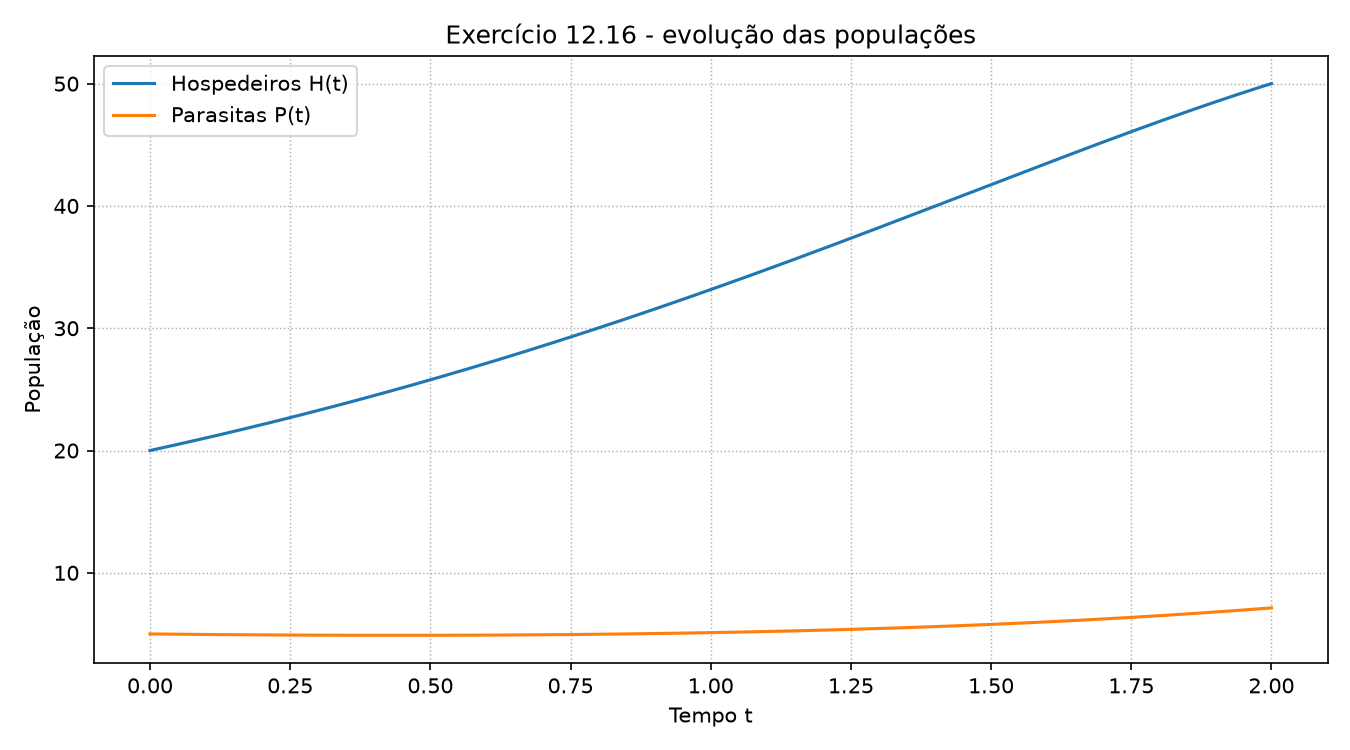
\includegraphics[width=0.85\textwidth]{../graficos/exercicio_12_16_evolucao.png}
    \caption{Evolução de hospedeiros e parasitas no Exercício 12.16.}
\end{figure}

\subsubsection{Avaliação no Modelo Epidêmico SEIAHR}

No modelo SEIAHR, a validação foi realizada pela coerência epidemiológica das curvas e pela comparação entre métodos. Usando a forma normalizada \(\lambda=\beta(I+A)/N\), o RK4 estimou, no dia 50, \(S=399943{,}190489\), \(I=4{,}891144\), \(H=0{,}025001\), \(R=28{,}369505\) e \(D=0{,}012338\). Os suscetíveis diminuem lentamente, enquanto recuperados e mortes acumuladas crescem sem oscilações artificiais.

Os compartimentos possuem interpretações distintas: \(S\) representa suscetíveis, \(E\) expostos, \(I\) infectados sintomáticos, \(A\) infectados assintomáticos, \(H\) hospitalizados, \(R\) recuperados e \(D\) mortes acumuladas. A variável \(D\) foi mantida separada de \(H\), pois hospitalização é um estado transitório, enquanto mortes acumuladas não decrescem. Com os parâmetros adotados, o número básico de reprodução calculado pela aproximação \(R_0=\beta(1-\chi)/\delta\) foi \(R_0=2{,}000000\).

\begin{table}[H]
    \centering
    \caption{Evolução selecionada do modelo SEIAHR normalizado pelo RK4.}
    \label{tab:seiahr-rk4-dias}
    \resizebox{\textwidth}{!}{
    \begin{tabular}{c|r|r|r|r|r|r|r}
        \textbf{Dia} & \textbf{\(S\)} & \textbf{\(E\)} & \textbf{\(I\)} & \textbf{\(A\)} & \textbf{\(H\)} & \textbf{\(R\)} & \textbf{\(D\)} \\
        \hline
        0 & 400000{,}000000 & 0{,}000000 & 1{,}000000 & 0{,}000000 & 0{,}000000 & 0{,}000000 & 0{,}000000 \\
        10 & 399997{,}881490 & 0{,}688128 & 0{,}618690 & 0{,}752431 & 0{,}003935 & 1{,}054528 & 0{,}000797 \\
        20 & 399993{,}992511 & 1{,}342445 & 0{,}766819 & 1{,}894451 & 0{,}004861 & 2{,}996806 & 0{,}002108 \\
        30 & 399986{,}434607 & 2{,}609504 & 1{,}330606 & 3{,}842455 & 0{,}007307 & 6{,}771650 & 0{,}003871 \\
        40 & 399971{,}743859 & 5{,}072205 & 2{,}527570 & 7{,}527762 & 0{,}013112 & 14{,}108669 & 0{,}006824 \\
        50 & 399943{,}190489 & 9{,}858308 & 4{,}891144 & 14{,}653217 & 0{,}025001 & 28{,}369505 & 0{,}012338 \\
    \end{tabular}}
\end{table}

A forma não normalizada \(\lambda=\beta(I+A)\) faz a força de infecção crescer diretamente com números absolutos de pessoas. Para uma população de \(400000\) indivíduos, essa formulação torna o sistema numericamente instável e epidemiologicamente menos plausível. A forma normalizada, por outro lado, expressa a fração efetiva de contatos infectantes e mantém as variáveis em escala compatível com a interpretação populacional.

\subsubsection{Conclusão Analítica Global dos Métodos de PVI}

A comparação confirma o comportamento teórico esperado. Euler é simples e didático, mas menos preciso. Heun e Ponto Médio apresentam ganho expressivo de precisão com pequeno aumento de custo. RK4 é o método mais robusto entre os testados, especialmente quando há crescimento acumulativo ou sistemas acoplados.

\section{Métodos para Problemas de Valor de Contorno}

Um Problema de Valor de Contorno, ou PVC, possui condições impostas em pontos distintos do domínio. Ao contrário dos PVIs, nos quais toda a informação inicial está concentrada em \(t_0\), no PVC parte da informação aparece no extremo final do intervalo. Essa diferença exige estratégias específicas de discretização ou transformação do problema.

\subsection{Método Shooting}

\subsubsection{Fundamentação Teórica}

O Método Shooting transforma um PVC em um PVI. No problema da haste, a equação

\[
    \frac{d^2T}{dx^2}=h'(T-T_a)
\]

foi reescrita como o sistema

\[
    \frac{dT}{dx}=z, \qquad \frac{dz}{dx}=h'(T-T_a).
\]

Como \(T(0)\) é conhecido, mas \(z(0)\) não é, escolhem-se chutes para a derivada inicial e corrige-se esse valor até satisfazer a condição \(T(10)=200\).

\subsubsection{Estratégia de Implementação}

Foram usados dois chutes iniciais para \(z(0)\). Cada chute foi integrado por RK4 de \(x=0\) a \(x=10\). Em seguida, aplicou-se interpolação linear para estimar o chute que faria a solução atingir a condição de contorno final.

\subsubsection{Estrutura dos Arquivos de Entrada e Saída}

Os parâmetros do problema estão em \texttt{exercicios/pvc/haste\_calor.py}. A saída numérica do Shooting foi salva em \texttt{resultados/pvc\_shooting.csv}, contendo \(x\), solução analítica, solução aproximada e erro absoluto.

\subsubsection{Problemas Teste}

\paragraph{Problema Teste 1: Condução de calor em uma haste}

O problema teste utilizado para o Método Shooting foi a condução de calor em uma haste com troca de calor com o ambiente. A equação diferencial de segunda ordem é

\[
    \frac{d^2T}{dx^2}=h'(T-T_a),
\]

com condições de contorno \(T(0)=40^\circ C\) e \(T(10)=200^\circ C\). Foram usados \(T_a=20^\circ C\), \(h'=0{,}01\) e comprimento \(L=10\). A solução analítica de referência é \(T(x)=73{,}4523e^{0{,}1x}-53{,}4523e^{-0{,}1x}+20\).

Para aplicar o Shooting, a equação de segunda ordem foi transformada em um sistema de primeira ordem, com \(dT/dx=z\) e \(dz/dx=h'(T-T_a)\). Como \(z(0)\) não é conhecido, foram usados dois chutes iniciais, \(z_1(0)=10\) e \(z_2(0)=20\). O primeiro chute produziu \(T(10)\approx168{,}381637\), abaixo da condição de contorno final; o segundo produziu \(T(10)\approx285{,}901673\), acima do valor desejado. Assim, a derivada inicial corrigida foi obtida por interpolação linear:

\[
    z(0)=z_1+\frac{T_L-T_{L,1}}{T_{L,2}-T_{L,1}}(z_2-z_1).
\]

\begin{table}[H]
    \centering
    \caption{Comparação ponto a ponto do Método Shooting no problema da haste.}
    \resizebox{\textwidth}{!}{
    \begin{tabular}{c|r|r|r}
        \textbf{\(x\)} & \textbf{Solução analítica} & \textbf{Shooting} & \textbf{Erro absoluto} \\
        \hline
        0{,}000000 & 40{,}000000 & 40{,}000000 & 0{,}000000 \\
        0{,}909091 & 51{,}635381 & 51{,}635379 & 0{,}000001 \\
        1{,}818182 & 63{,}532391 & 63{,}532388 & 0{,}000003 \\
        2{,}727273 & 75{,}789421 & 75{,}789416 & 0{,}000005 \\
        3{,}636364 & 88{,}507839 & 88{,}507831 & 0{,}000007 \\
        4{,}545455 & 101{,}792826 & 101{,}792816 & 0{,}000010 \\
        5{,}454545 & 115{,}754254 & 115{,}754240 & 0{,}000014 \\
        6{,}363636 & 130{,}507583 & 130{,}507565 & 0{,}000019 \\
        7{,}272727 & 146{,}174828 & 146{,}174804 & 0{,}000024 \\
        8{,}181818 & 162{,}885559 & 162{,}885527 & 0{,}000031 \\
        9{,}090909 & 180{,}777975 & 180{,}777935 & 0{,}000040 \\
        10{,}000000 & 200{,}000050 & 200{,}000000 & 0{,}000050 \\
    \end{tabular}}
\end{table}
% TODO: inserir figura específica do Método Shooting no problema da haste

O resultado final respeitou as condições de contorno e apresentou erro máximo de \(0{,}000050\) em relação à solução analítica. A precisão observada indica que a combinação entre Shooting, RK4 e interpolação linear foi adequada para este problema.

\subsubsection{Validação dos Resultados}

A validação foi conduzida por comparação com a solução analítica

\[
    T(x)=73{,}4523e^{0{,}1x}-53{,}4523e^{-0{,}1x}+20.
\]

O erro máximo do Shooting foi \(0{,}000050\), e o erro médio foi aproximadamente \(0{,}000017\). Além disso, a solução respeitou as condições de contorno, atingindo \(T(0)=40\) e \(T(10)=200\).

\subsubsection{Dificuldades Enfrentadas}

A dificuldade central foi determinar a derivada inicial desconhecida. Um chute inadequado não invalida o método, mas exige correção cuidadosa. A interpolação linear entre dois chutes tornou o procedimento estável para o problema analisado.

\subsection{Método das Diferenças Finitas}

\subsubsection{Fundamentação Teórica}

O Método das Diferenças Finitas substitui derivadas por aproximações algébricas. Para a segunda derivada, usou-se

\[
    \frac{d^2T}{dx^2}\approx\frac{T_{i+1}-2T_i+T_{i-1}}{\Delta x^2}.
\]

Substituindo essa aproximação na equação da haste, obtém-se um sistema linear tridiagonal para os pontos internos.

\subsubsection{Estratégia de Implementação}

O intervalo \([0,10]\) foi dividido em 11 subintervalos, gerando 10 pontos internos. A matriz tridiagonal foi resolvida manualmente pelo algoritmo de Thomas, sem uso de \texttt{numpy.linalg.solve} ou de qualquer biblioteca pronta para sistemas lineares.

\subsubsection{Estrutura dos Arquivos de Entrada e Saída}

Os dados do problema são os mesmos utilizados no Shooting. A tabela de saída foi salva em \texttt{resultados/pvc\_diferencas\_finitas.csv}, contendo posição, solução analítica, solução aproximada e erro absoluto.

\subsubsection{Problemas Teste}

\paragraph{Problema Teste 1: Condução de calor em uma haste}

O problema teste do Método das Diferenças Finitas foi o mesmo problema de condução de calor na haste, com \(T(0)=40^\circ C\), \(T(10)=200^\circ C\), \(T_a=20^\circ C\), \(h'=0{,}01\) e \(L=10\). A equação diferencial considerada foi

\[
    \frac{d^2T}{dx^2}=h'(T-T_a).
\]

O domínio foi discretizado com 10 pontos internos, isto é, o intervalo \([0,10]\) foi dividido em 11 subintervalos. A segunda derivada foi aproximada por diferenças centradas, produzindo um sistema linear tridiagonal. As condições de contorno foram incorporadas no primeiro e no último termos independentes do sistema.

Com \(\Delta x=10/11\), o sistema interno possui diagonal principal \(2+h'\Delta x^2\), subdiagonal \(-1\), superdiagonal \(-1\) e vetor de termos independentes iniciado por \(h'\Delta x^2T_a+T(0)\) e finalizado por \(h'\Delta x^2T_a+T(10)\). Essa estrutura tridiagonal justifica o uso do algoritmo de Thomas.

\begin{table}[H]
    \centering
    \caption{Comparação ponto a ponto das Diferenças Finitas no problema da haste.}
    \resizebox{\textwidth}{!}{
    \begin{tabular}{c|r|r|r}
        \textbf{\(x\)} & \textbf{Solução analítica} & \textbf{Diferenças finitas} & \textbf{Erro absoluto} \\
        \hline
        0{,}000000 & 40{,}000000 & 40{,}000000 & 0{,}000000 \\
        0{,}909091 & 51{,}635381 & 51{,}637179 & 0{,}001799 \\
        1{,}818182 & 63{,}532391 & 63{,}535823 & 0{,}003432 \\
        2{,}727273 & 75{,}789421 & 75{,}794267 & 0{,}004846 \\
        3{,}636364 & 88{,}507839 & 88{,}513821 & 0{,}005982 \\
        4{,}545455 & 101{,}792826 & 101{,}799604 & 0{,}006778 \\
        5{,}454545 & 115{,}754254 & 115{,}761417 & 0{,}007164 \\
        6{,}363636 & 130{,}507583 & 130{,}514647 & 0{,}007064 \\
        7{,}272727 & 146{,}174828 & 146{,}181221 & 0{,}006393 \\
        8{,}181818 & 162{,}885559 & 162{,}890615 & 0{,}005057 \\
        9{,}090909 & 180{,}777975 & 180{,}780924 & 0{,}002949 \\
        10{,}000000 & 200{,}000050 & 200{,}000000 & 0{,}000050 \\
    \end{tabular}}
\end{table}
% TODO: inserir figura específica das Diferenças Finitas no problema da haste

A solução do sistema foi obtida manualmente pelo algoritmo de Thomas. O erro máximo em relação à solução analítica foi \(0{,}007164\), e o erro médio foi \(0{,}004293\). O resultado acompanha a tendência crescente da temperatura ao longo da haste, preservando coerência física e respeitando as condições de contorno.

\subsubsection{Validação dos Resultados}

A validação foi feita pela comparação com a solução analítica e com o método Shooting. O erro máximo das Diferenças Finitas foi \(0{,}007164\), e o erro médio foi \(0{,}004293\). Os valores respeitaram as condições de contorno e acompanharam a tendência crescente da temperatura ao longo da haste.

\subsubsection{Dificuldades Enfrentadas}

O principal cuidado foi incorporar corretamente as condições de contorno no primeiro e no último ponto interno. Outro ponto importante foi resolver o sistema tridiagonal manualmente, preservando a restrição de não usar bibliotecas prontas.

\subsection{Análise Comparativa dos Métodos para Problemas de Valor de Contorno}

\subsubsection{Avaliação do problema da haste com 10 pontos internos}

Com 10 pontos internos, ambos os métodos produziram soluções próximas da solução analítica. O Shooting apresentou erro médio menor, enquanto as Diferenças Finitas mantiveram boa consistência global.

\subsubsection{Comparação entre Shooting e Diferenças Finitas}

O Shooting apresentou erro máximo de \(0{,}000050\), contra \(0{,}007164\) das Diferenças Finitas. Nesse teste, portanto, o Shooting aproximou melhor a solução analítica. No entanto, as Diferenças Finitas oferecem uma estrutura mais direta para problemas em que a discretização espacial é o foco principal.

\begin{figure}[H]
    \centering
    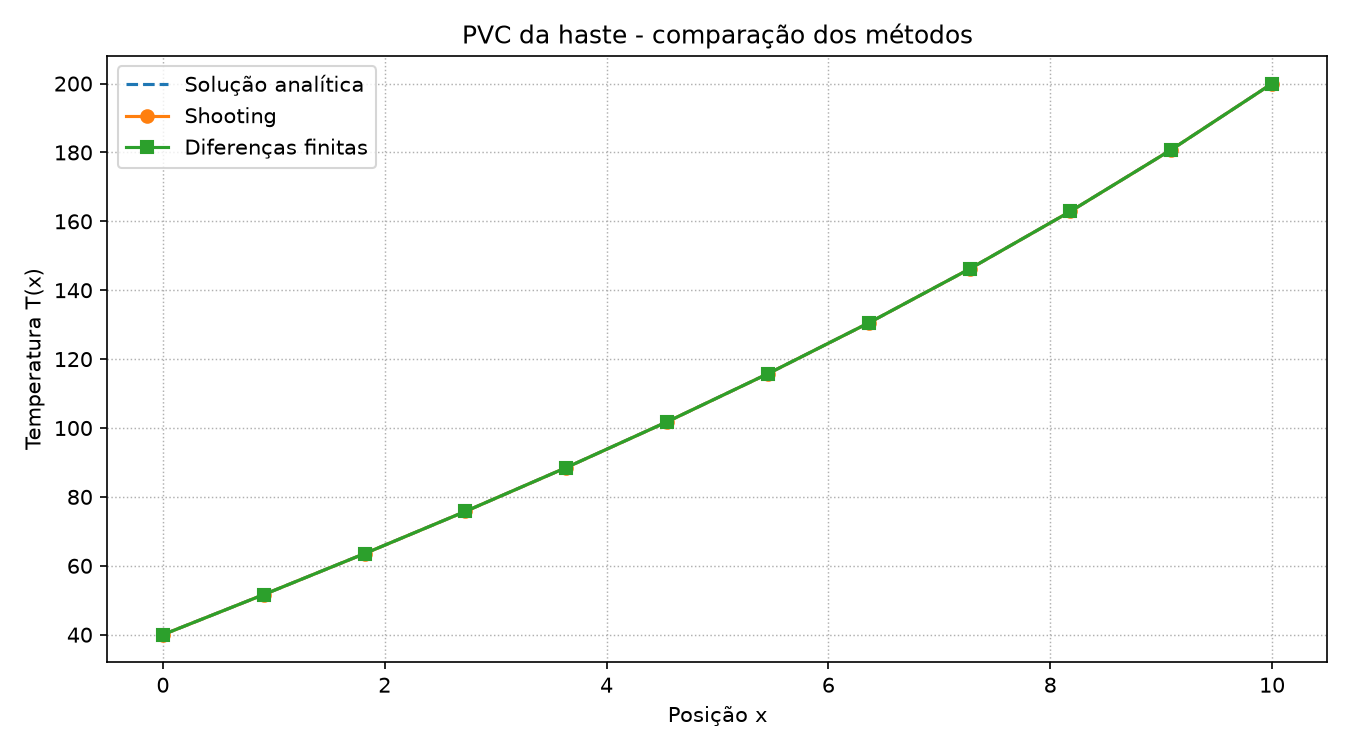
\includegraphics[width=0.85\textwidth]{../graficos/pvc_comparacao.png}
    \caption{Comparação entre solução analítica, Shooting e Diferenças Finitas.}
\end{figure}

\begin{table}[H]
    \centering
    \caption{Comparação ponto a ponto entre Shooting e Diferenças Finitas.}
    \resizebox{\textwidth}{!}{
    \begin{tabular}{c|r|r|r|r}
        \textbf{\(x\)} & \textbf{Solução analítica} & \textbf{Shooting} & \textbf{Diferenças finitas} & \textbf{Erro DF} \\
        \hline
        0{,}000000 & 40{,}000000 & 40{,}000000 & 40{,}000000 & 0{,}000000 \\
        0{,}909091 & 51{,}635381 & 51{,}635379 & 51{,}637179 & 0{,}001799 \\
        1{,}818182 & 63{,}532391 & 63{,}532388 & 63{,}535823 & 0{,}003432 \\
        2{,}727273 & 75{,}789421 & 75{,}789416 & 75{,}794267 & 0{,}004846 \\
        3{,}636364 & 88{,}507839 & 88{,}507831 & 88{,}513821 & 0{,}005982 \\
        4{,}545455 & 101{,}792826 & 101{,}792816 & 101{,}799604 & 0{,}006778 \\
        5{,}454545 & 115{,}754254 & 115{,}754240 & 115{,}761417 & 0{,}007164 \\
        6{,}363636 & 130{,}507583 & 130{,}507565 & 130{,}514647 & 0{,}007064 \\
        7{,}272727 & 146{,}174828 & 146{,}174804 & 146{,}181221 & 0{,}006393 \\
        8{,}181818 & 162{,}885559 & 162{,}885527 & 162{,}890615 & 0{,}005057 \\
        9{,}090909 & 180{,}777975 & 180{,}777935 & 180{,}780924 & 0{,}002949 \\
        10{,}000000 & 200{,}000050 & 200{,}000000 & 200{,}000000 & 0{,}000050 \\
    \end{tabular}}
\end{table}

\subsubsection{Conclusão Analítica Global dos Métodos de PVC}

Os dois métodos validam a solução do problema de contorno, mas partem de ideias diferentes. O Shooting depende de transformar o PVC em PVI e ajustar a derivada inicial. As Diferenças Finitas substituem a equação diferencial por um sistema algébrico. No problema da haste, o Shooting foi numericamente mais preciso, mas ambos apresentaram comportamento físico coerente.

\section{Organização Geral da Implementação}

\subsection{Modularização do Código}

O projeto foi organizado de forma modular. Os métodos numéricos estão em \texttt{metodos/}; as definições dos problemas estão em \texttt{exercicios/}; a execução geral fica em \texttt{main.py}; e as funções auxiliares de escrita de arquivos estão em \texttt{utils.py}.

\begin{lstlisting}
metodos/
  pvi.py
  sistemas.py
  pvc.py
exercicios/
  pvi/
  sistemas/
  seiahr/
  pvc/
resultados/
graficos/
explicacoes/
relatorio/
\end{lstlisting}

Essa organização separa a formulação dos métodos, a definição dos problemas e a geração dos artefatos usados no relatório. Com isso, o mesmo método pode ser reutilizado em diferentes exercícios sem duplicar código.

\subsection{Arquivos de Entrada}

Os arquivos de entrada são módulos Python contendo parâmetros, funções diferenciais, condições iniciais e soluções analíticas quando disponíveis. Essa escolha evita leitura manual de dados e facilita a reprodução dos experimentos.

\subsection{Arquivos de Saída}

As tabelas foram gravadas na pasta \texttt{resultados/}, em CSV com codificação UTF-8. Os textos explicativos foram salvos em \texttt{explicacoes/}, e os gráficos em \texttt{graficos/}.

\subsection{Geração de Tabelas}

As tabelas incluem valores aproximados, solução exata quando disponível, erro absoluto e erro relativo. Essa organização permite validar os métodos quantitativamente, e não apenas por inspeção visual.

\subsection{Geração de Gráficos}

Os gráficos foram gerados com \texttt{matplotlib}. Eles foram usados para comparar soluções numéricas, observar evolução temporal de variáveis e verificar visualmente a coerência dos resultados.

\begin{figure}[H]
    \centering
    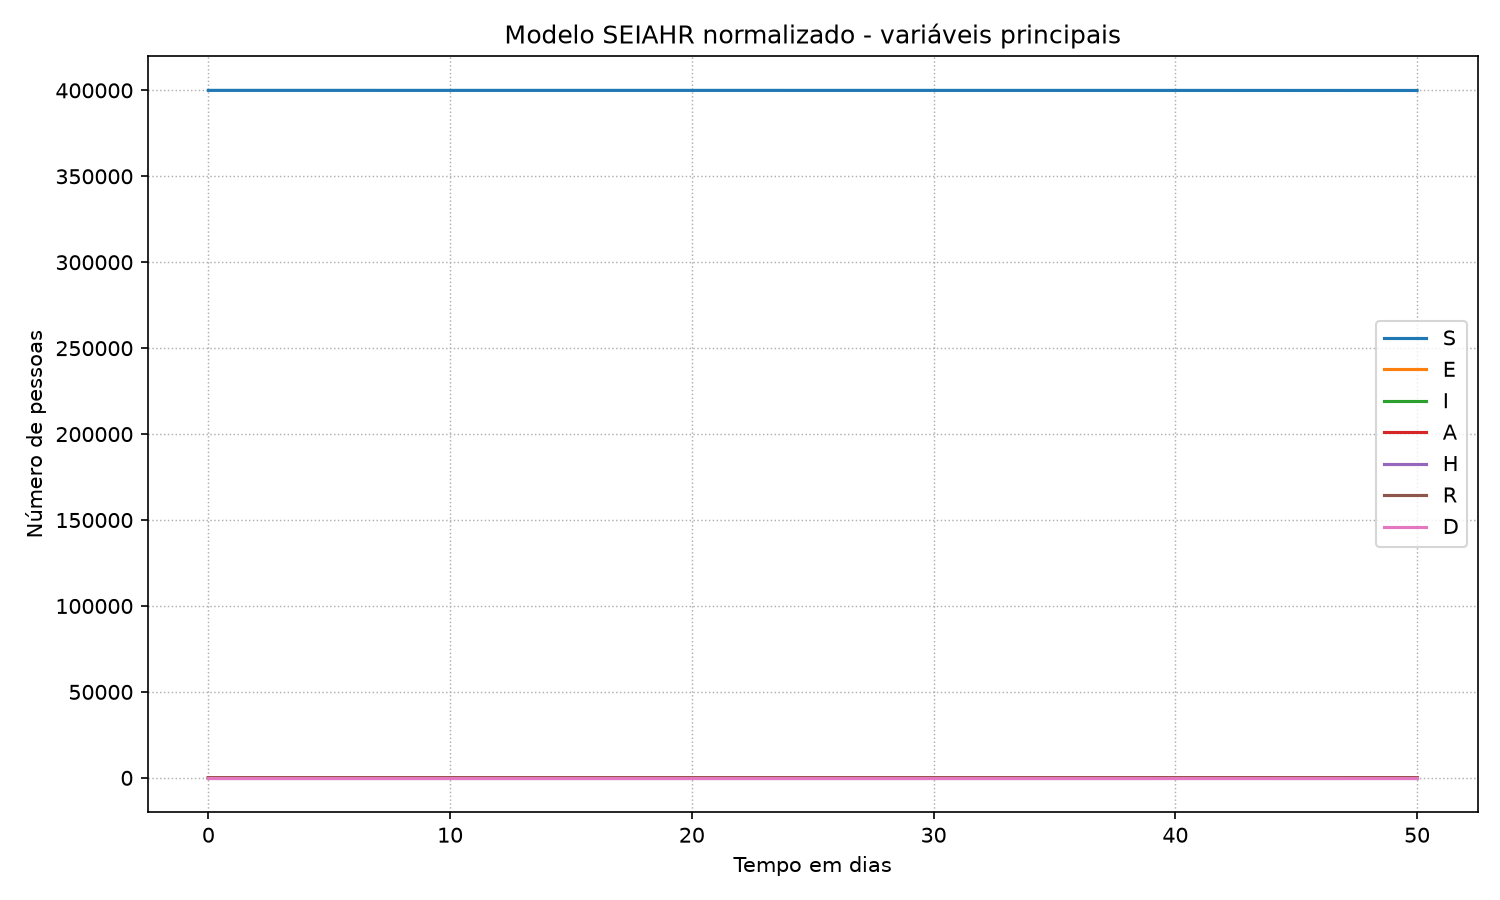
\includegraphics[width=0.85\textwidth]{../graficos/seiahr_comparativo.png}
    \caption{Evolução das variáveis do modelo SEIAHR normalizado.}
\end{figure}

% TODO: inserir gráficos de erro específicos para cada método, caso sejam exigidos em versão final.

\subsection{Restrições de Implementação}

Não foram usados \texttt{numpy}, \texttt{pandas}, \texttt{scipy}, solucionadores prontos de EDOs ou rotinas prontas para sistemas lineares. Todos os métodos foram implementados manualmente, incluindo o algoritmo de Thomas usado nas Diferenças Finitas.

\section{Considerações Finais}

O relatório foi organizado por tipo de método e por método numérico, de modo que os exercícios aparecem como problemas teste e não como eixos principais da exposição. Essa organização evidencia melhor a função de cada método, sua fundamentação, sua implementação e seus critérios de validação.

Nos Problemas de Valor Inicial, os resultados confirmaram a relação entre ordem do método e precisão. Euler foi o método mais simples e menos preciso. Heun e Ponto Médio apresentaram ganho significativo de qualidade com custo moderado. RK4 foi o método mais preciso e estável entre os testados, especialmente em problemas com solução analítica e em sistemas acoplados.

Nos Problemas de Valor de Contorno, Shooting e Diferenças Finitas produziram aproximações coerentes. O Shooting apresentou menor erro no problema da haste, enquanto as Diferenças Finitas demonstraram a utilidade da discretização do domínio e da resolução manual de sistemas tridiagonais.

De modo geral, a implementação manual dos métodos permitiu relacionar diretamente teoria, código e validação numérica. Essa relação é essencial em Métodos Numéricos, pois o resultado computacional só é confiável quando acompanhado de análise de erro, interpretação do comportamento da solução e verificação da consistência matemática do procedimento utilizado.
